\documentclass[10pt]{extarticle}

% Lingua e matematica
\usepackage[english]{babel}
\usepackage{amsmath,amssymb,amsthm}

% Grafica e tabelle
\usepackage{graphicx}
\usepackage{subcaption}
\usepackage{float}
\usepackage{booktabs}
\usepackage{multirow}
\usepackage{siunitx}

% Codice (opzionale)
\usepackage{listings}
\usepackage{xcolor}
\definecolor{codegreen}{rgb}{0,0.6,0}
\definecolor{codegray}{rgb}{0.5,0.5,0.5}
\definecolor{codepurple}{rgb}{0.58,0,0.82}
\definecolor{backcolour}{rgb}{0.98,0.98,0.98}
\lstdefinestyle{mystyle}{
  backgroundcolor=\color{backcolour},
  commentstyle=\color{codegreen},
  keywordstyle=\color{magenta},
  numberstyle=\tiny\color{codegray},
  stringstyle=\color{codepurple},
  basicstyle=\ttfamily\footnotesize,
  breaklines=true, keepspaces=true, numbers=none, tabsize=2
}
\lstset{style=mystyle}

% Margini
\usepackage[margin=0.6in]{geometry}
\usepackage{ragged2e}
\usepackage{enumitem}
%\usepackage[utf8]{inputenc} % per caratteri UTF-8 nei .tex e nel .bib
\usepackage[backend=biber,style=ieee,sorting=none,maxbibnames=99]{biblatex}
\ExecuteBibliographyOptions{doi=true,url=true,isbn=false}
\addbibresource{references.bib}
\usepackage{csquotes}       % consigliato da biblatex (evita warning e parse strani)



% Bibliografia (biblatex + biber)
\usepackage[backend=biber,style=ieee]{biblatex}
\addbibresource{references.bib}

% TOC: includi anche \paragraph e numerali
\setcounter{secnumdepth}{2}
\setcounter{tocdepth}{2}

% Hyperref (sempre *dopo* gli altri pacchetti)
\usepackage[colorlinks=true,linkcolor=blue,citecolor=teal,urlcolor=magenta]{hyperref}


\begin{document}

% Custom header without a separate titlepage
\noindent
\begin{minipage}{0.3\textwidth}
    
\includegraphics[width=1.3\linewidth]{Figures/polito_logo_2021_blu.jpg}
\end{minipage}
\hfill
\begin{minipage}{0.68\textwidth}
    \raggedleft
    {\LARGE \textbf{Politecnico di Torino}}\\[0.2cm]
    {\large Master's Degree in Mathematical Engineering}\\[0.7cm]
    {\large \textbf{Material for Thesis}}\\[0.2cm]
    {\large 3-- About Data pre-processing}\\[0.7cm]
    \begin{tabular}{rl}
        Elisabetta Roviera & \texttt{s328422} \\
    \end{tabular}
\end{minipage}

\vspace{1cm}
\hrule
\vspace{0.5cm}

\tableofcontents

\vspace{0.5cm}
\hrule
\vspace{1cm}


% Main content begins here, on the same page
\justifying

\paragraph{Note} 
The papers summarized in this report currently represent the main references consulted for the data pre-processing stage of the thesis, with a focus on methodologies for methylation array normalization, probe filtering, and batch-effect correction. Additional studies may be reviewed in the future to refine specific analytical or computational aspects. For a comprehensive understanding of the methods and results discussed, consult the original publications, all of which are cited in the bibliography of this document.

\section{Comparison of Beta-value and M-value methods for quantifying methylation levels by microarray analysis}

\paragraph{Keywords} DNA methylation, Beta-value, M-value, Illumina Infinium, variance stabilization, effect size, statistical modeling \cite{Du2010}

\paragraph{Introduction}
The study focuses on two alternative measures for quantifying CpG methylation signals obtained from Illumina Infinium microarray platforms. Although both metrics rely on the same methylated (M) and unmethylated (U) probe intensities, they differ in scale, statistical behavior, and suitability for downstream analysis. The objective is to determine which representation is more appropriate for differential methylation studies and to clarify their interpretation, transformation, and practical use.

\paragraph{Definition of Beta-value}
The Beta-value estimates the proportion of methylated signal and is defined as:
\[
\beta_i = \frac{\max(y^{(M)}_i, 0)}{\max(y^{(M)}_i, 0) + \max(y^{(U)}_i, 0) + \alpha}
\]
where \(y^{(M)}_i\) and \(y^{(U)}_i\) are background-corrected intensities, and \(\alpha\) is a small constant used to avoid division by zero. The resulting value lies in the interval \([0,1]\) and is often interpreted as the percentage of methylation at a locus. While intuitive, the bounded nature of the Beta-value causes compression at the extremes, reducing the ability to detect differences in highly or weakly methylated regions. Figure \ref{fig:M_value_vs_B_value} visually illustrates how the transformation flattens values close to 0 and 1.


\paragraph{Definition of M-value}
The M-value is a log-ratio that transforms the same intensities onto an unbounded scale:
\[
M_i = \log_2 \left( \frac{\max(y^{(M)}_i, 0) + \alpha}{\max(y^{(U)}_i, 0) + \alpha} \right)
\]
Values around zero indicate approximately half-methylation, while positive or negative values reflect higher methylation or unmethylation, respectively. Because the M-value is not constrained to a fixed range, it expands differences at the extremes and supports assumptions of normality more effectively. The inverse logit relation between the two metrics explains why the M-value preserves variation in regions where the Beta-value loses resolution. Figure \ref{fig:M_value_vs_B_value} also highlights this link.

\begin{figure}[h]
    \centering
    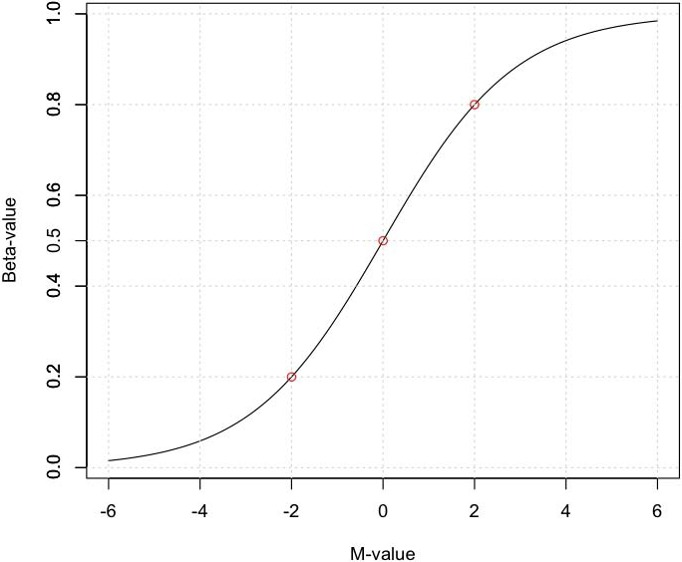
\includegraphics[width=0.3\textwidth]{Figures/The relationship curve between M-value and Betavalue.jpg} % o .png, .pdf, .eps...
    \caption{The relationship curve between M-value and Betavalue.}
    \label{fig:M_value_vs_B_value}
\end{figure}

\paragraph{Statistical Comparison}
A central focus of the paper is how the two metrics behave when used for differential methylation analysis. Beta-values display heteroscedasticity, meaning that their variance depends strongly on the mean. In particular, values close to the boundaries show lower variability and greater compression. This poses a challenge for tests that assume equal variance across groups. The M-value, due to its log-ratio nature, results in variance that is roughly constant along the entire range of methylation. This homoscedasticity makes it more suitable for parametric models and t-statistics commonly used in genomics.

The authors emphasize that the difference in variance structure directly affects effect-size estimation. For Beta-values, a 5\% change near 0.5 is not equivalent to a 5\% change near 0.95. The M-value preserves differences more uniformly across the entire spectrum. Figure \ref{fig:histo_M_value_vs_B_value} shows how M-values more clearly reflect bimodal distributions of methylation states, revealing biological patterns that the Beta-value can obscure. Figure \ref{fig:mean_std_M_value_vs_B_value} further demonstrates the contrast in variance, showing increasing instability in Beta-values compared to the stable behavior of M-values.

\begin{figure}[h]
    \centering
    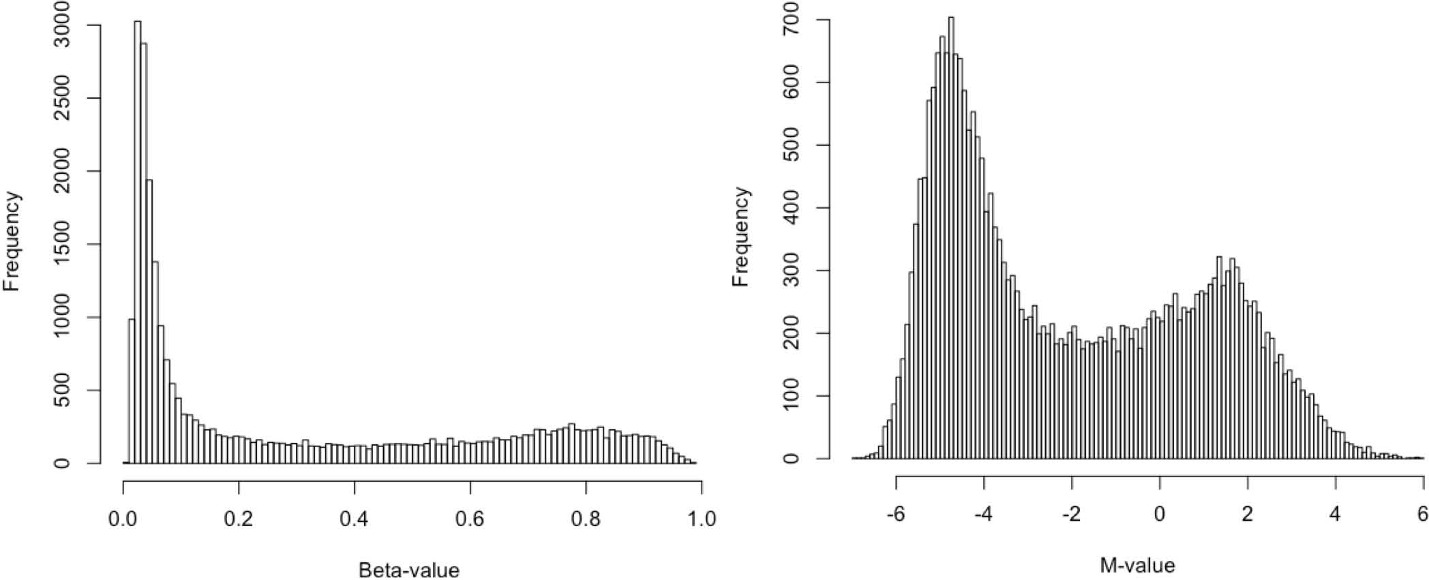
\includegraphics[width=0.7\textwidth]{Figures/The histograms of Beta-value (left) and M-value (right) (27578 interrogated CpG sites in total)..jpg} % o .png, .pdf, .eps...
    \caption{The histograms of Beta-value (left) and M-value (right) (27578 interrogated CpG sites in total).}
    \label{fig:histo_M_value_vs_B_value}
\end{figure}

\begin{figure}[h]
    \centering
    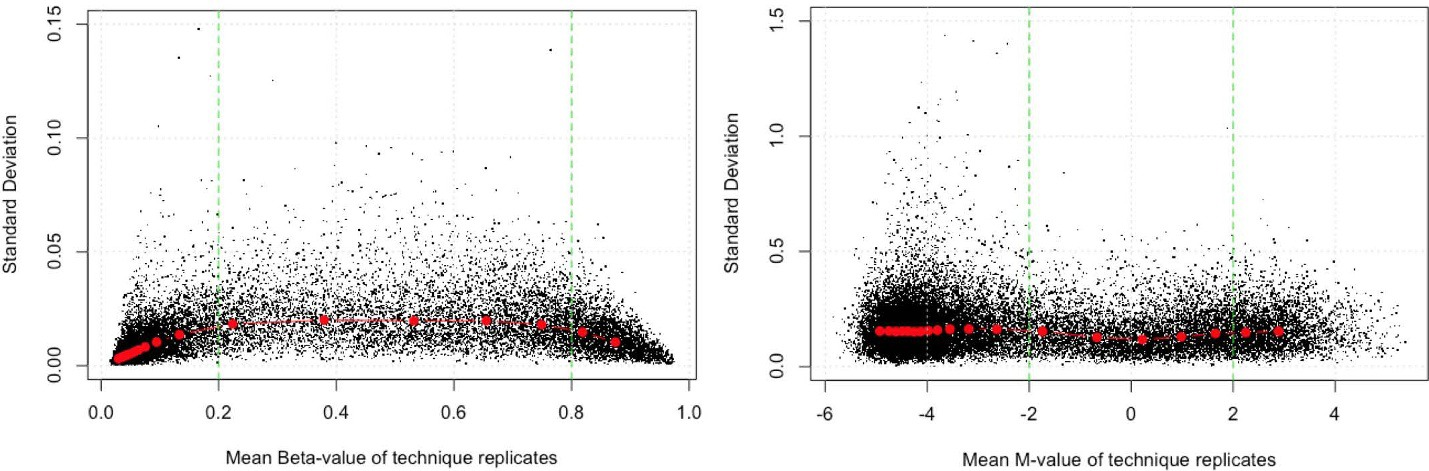
\includegraphics[width=0.7\textwidth]{Figures/The mean and standard deviation relations of technical replicates. Beta-value (left) and M-value (right).jpg} % o .png, .pdf, .eps...
    \caption{The mean and standard deviation relations of technical replicates. Beta-value (left) and M-value (right)The mean and standard deviation relations of technical replicates. Beta-value (left) and M-value (right).}
    \label{fig:mean_std_M_value_vs_B_value}
\end{figure}



\paragraph{Additional Comparative Insights}
The comparison goes beyond variance and range. The authors underline that Beta-values are more appropriate when the primary objective is to communicate methylation status as a proportion or visualize relative differences. However, when applying linear models or ranking CpG sites based on effect sizes, M-values outperform Beta-values because of the stabilized variance and symmetrical distribution. The paper discusses how ranking CpGs by absolute differences in M-values captures signals effectively across all methylation levels, while Beta-values fail to do so consistently at the boundaries.

Another key point is that global thresholds applied to Beta-values may not capture meaningful differences in hyper- or hypo-methylated regions. In contrast, M-values allow a more uniform threshold that applies across ranges without losing sensitivity. This distinction is essential for studies involving differential methylation between biological groups, where overestimation or underdetection of CpGs can bias conclusions.

\paragraph{Figure Insights}
Figure \ref{fig:M_value_vs_B_value} illustrates the non-linear transformation between Beta-values and M-values and highlights how the M-value de-compresses signals in the extreme ranges. Figure \ref{fig:histo_M_value_vs_B_value} shows that the M-value better visualizes bimodal methylation distributions, while the Beta-value compresses them toward the boundaries. Figure \ref{fig:mean_std_M_value_vs_B_value} focuses on the variance structure, demonstrating that Beta-values become unstable and non-homogeneous across the methylation range, whereas M-values maintain approximate variance consistency. These three figures provide the conceptual basis for understanding why downstream analyses can yield different results depending on the chosen metric.

\paragraph{Conclusions}
The paper concludes that the M-value is superior for statistical inference, particularly when identifying differentially methylated CpG sites. Its unbounded nature, variance stabilization, and compatibility with linear-model frameworks make it more appropriate for hypothesis testing and effect-size ranking. Beta-values remain useful for interpretation and presentation because they directly approximate methylation proportions. A practical approach is to conduct statistical testing in M-value space and convert results back to Beta-values for visualization or reporting. The findings emphasize that choosing the appropriate metric affects sensitivity, variance handling, and interpretability in methylation studies, especially when working with high-throughput microarray data.

\section{Reducing the risk of false discovery enabling identification of biologically significant genome-wide methylation status using the HumanMethylation450 array}

\paragraph{Keywords} HumanMethylation450K BeadChip, SNPs, INDELS, Repetitive regions of DNA, SNP arrays, HM450K bead
array, Epigenome-wide association studies, EWAS, Cancer, Epigenetics \cite{naeem2014}

\paragraph{Background and motivation}
The Illumina HumanMethylation450K (HM450K) array assays \(\sim\)485{,}000 CpGs genome-wide and is widely used in large cohorts due to its cost and throughput. However, non-methylation genomic factors can distort probe hybridization and base ligation, introducing spurious methylation signals. These factors include: (i) single nucleotide polymorphisms (SNPs), (ii) short insertions/deletions (INDELs), (iii) repetitive DNA, and (iv) multi-mapping of probes in the bisulfite-converted genome, which has reduced sequence complexity. The study systematically quantifies these effects by benchmarking HM450K \(\beta\) values against whole-genome bisulfite sequencing (WGBS) and derives a principled filtering strategy that maximizes true signal while minimizing noise. 

\paragraph{Data and gold standard comparison}
The authors compare HM450K measurements to matched WGBS in H1-hESC (ENCODE), profile 63 ENCODE cell lines, analyze primary prostate tumors vs. benign tissue, and evaluate blood cohorts to characterize within-tissue variability. High-quality probes (unaffected by known confounders) show very high correlation with WGBS (Infinium I \(r{=}0.95\); Infinium II \(r{=}0.92\)), establishing an empirical background error for subsequent tests of probe categories. 

\paragraph{Probe categories and headline counts}
Across 485{,}512 probes, the authors quantify potentially problematic classes: multi-mapping (\(\sim\)19{,}834), repeats (\(\sim\)38{,}743), SNP at the interrogated CpG (\(\sim\)70{,}118), and other SNP/INDEL contexts. If one removed \emph{all} potentially affected probes, only \(\sim\)172{,}587 would remain; however, the evidence-based filtering rescues many probes and retains \(\sim\)294{,}840 (keeping 60\% of the array) while discarding \(\sim\)39\%.

\paragraph{Filtering workflow (decision logic)}
The pre-processing proceeds in stages before methylation calling:
\begin{enumerate}
  \item \textbf{Uniqueness in bisulfite space}: build a “bisulfite genome” (C\(\to\)T) and remove probes mapping to multiple loci (ambiguous methylation source). 
  \item \textbf{Repetitive elements}: remove probes overlapping RepeatMasker-annotated repeats, which show the largest WGBS–array \(\beta\) discrepancies. 
  \item \textbf{INDEL overlaps}: annotate with dbSNP; INDEL-overlapping probes are generally \emph{kept} by default because their performance vs. high-quality probes is similar, with caveats by study design (population-wide vs. homogeneous systems). 
  \item \textbf{SNP overlaps}: annotate with dbSNP; if no SNP is present, keep; if present, apply rules in steps 5–6. 
  \item \textbf{SNP at the interrogated CpG}: remove, as this can abolish/alter the CpG itself and markedly inflate \(\beta\) error. 
  \item \textbf{“Bisulfite-OK” SNPs}: tolerate C\(\leftrightarrow\)T changes outside CpGs (always read as T after bisulfite) when the downstream neighbor is not G; these variants do not measurably degrade performance. 
\end{enumerate}

\begin{figure}[h]
  \centering
  % Replace the filename below with the actual path to Figure 4 (panel a/b) from the paper
  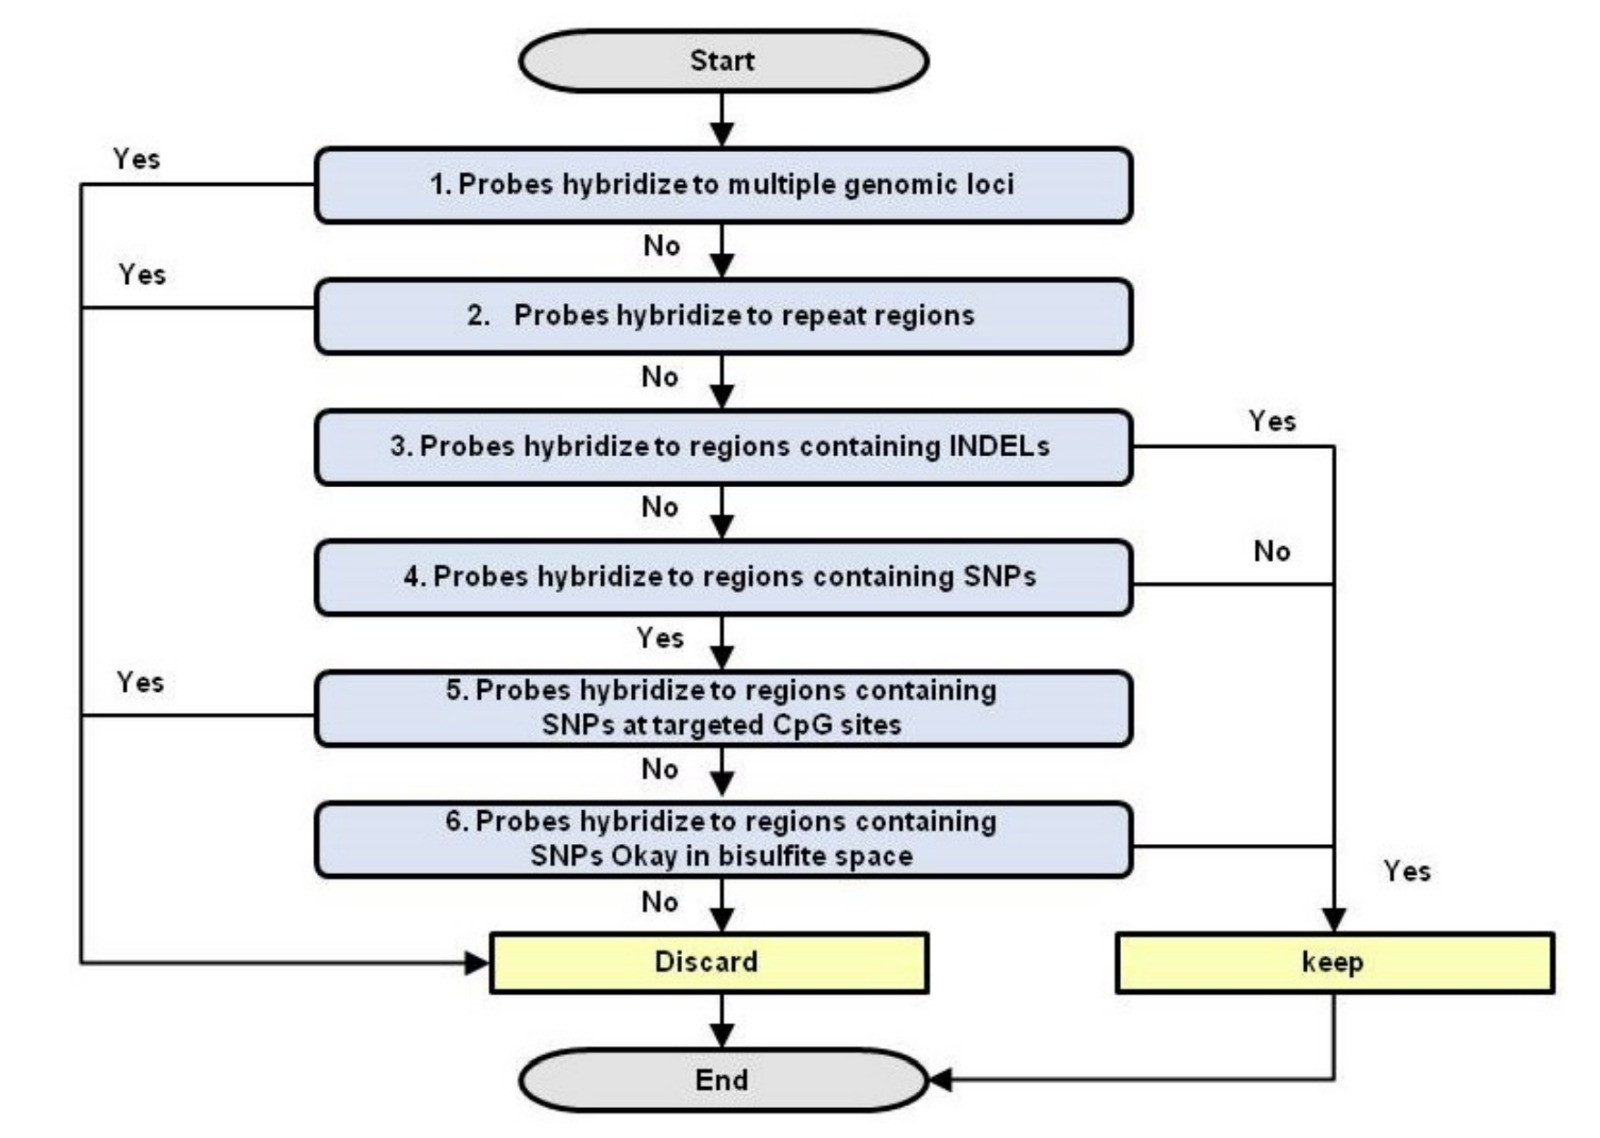
\includegraphics[width=0.7\linewidth]{Figures/Workflow for determining affected Probes..jpg}
  \caption{In step (1) the probes which were
not aligned to unique, unambiguous loci in the human genome were discarded. In step (2),
probes which hybridize to regions overlapped with repetitive DNA regions were discarded.
In step (3), probes which hybridize to regions containing only known indels that is, they
represent the insertion or deletion of one or multiple nucleotides were kept for the
subsequent analysis. Next (step 4), the SNP-containing probes have been marked and
subjected for downstream filtering analysis (Steps (5-6)). First, the probes which hybridize to
regions containing known SNP at the interrogated CpG sites were discarded (step 5). Then,
the probes which were unlikely to be affected by those SNPs that were okay in bisulphitetreated genome space (step 6), kept for further analysis.}
  \label{fig:Workflow}
\end{figure}



\paragraph{Kept vs. discarded probes (final tallies)}
The recommended filter removes 190{,}672 probes (39\%) and keeps 294{,}840, including 172{,}587 high-quality probes plus 122{,}253 “rescued” probes that evidence shows are not noisy despite initial flags. This balance preserves broad genomic coverage; the main depletion occurs in a few regions (e.g., HLA on chr6) and CpG island “shelves,” while islands and many functional categories remain well covered. 

\paragraph{Effect on downstream biology}
When applied to prostate tumor vs. benign tissue, filtering shifts differential-methylation results toward more biologically coherent networks. Without filtering, top networks are ribosomal; with the recommended filter, the androgen receptor (AR) network emerges, matching prostate cancer biology and therapy relevance—an effect obscured without principled filtering. 

\paragraph{Figure \ref{fig:std} within-tissue variability after filtering}
The study compares the \emph{within-tissue standard deviation (SD)} of \(\beta\) across probe sets: ALL, KEEP, and DISCARD, in blood datasets (4 samples and an independent 261-sample subset). The \textbf{KEEP} set exhibits significantly lower SD than \textbf{DISCARD}, indicating that filtered probes reduce technical noise and enhance statistical power in downstream analyses (e.g., differential methylation). Reported Wilcoxon \(p\)-values confirm the shift toward lower dispersion in KEEP. 

\begin{figure}[h]
  \centering
  % Replace the filename below with the actual path to Figure 4 (panel a/b) from the paper
  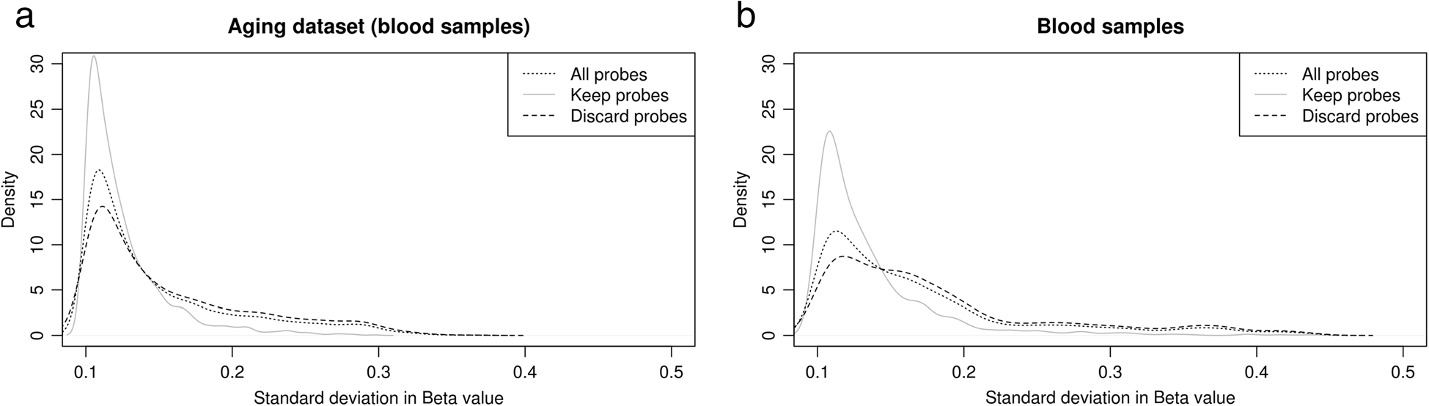
\includegraphics[width=0.9\linewidth]{Figures/This figure shows the distribution of standard deviation in beta values for probes on HM450K bead array, using (a) 4 blood.jpg}
  \caption{This figure shows the distribution of standard deviation in beta values for probes on HM450K bead array, using (a) 4 blood
samples and (b) 261 blood samples. In each case, the distribution of standard deviation in beta values ($\geq$ 0.10) was plotted for all probes, for
probes kept for subsequent analysis (Keep probes), and for the recommended removal of probes (Discard probes).}
  \label{fig:std}
\end{figure}

\paragraph{Design choices, caveats, and flexibility}
Because noise sources can be platform- and cohort-specific, the authors emphasize that thresholds and rescue rules may be tuned to study goals (e.g., population diversity, availability of genotypes). For instance, Infinium I probes are more sensitive to SNPs in the probe body, whereas Infinium II can tolerate \(\geq\)2 SNPs due to degenerate bases at CpGs; yet SNPs \emph{at} the interrogated CpG remain problematic across chemistries. Average SNP heterozygosity is not generally useful unless matched to the target population. 

\section{Comparison of pre-processing methodologies for Illumina 450k methylation array data in familial analyses}

\textbf{Keywords:} Familial data, 450k array, DNA methylation, pre-processing, normalization, ComBat, stratified quantile normalization \cite{Cazaly2016}.

\paragraph{Background}
The study addresses the challenges of DNA methylation data preprocessing in familial contexts using the Illumina HumanMethylation450 BeadChip (450k array). Unlike traditional case-control or tumor-normal designs, familial analyses lack clear reference samples, complicating normalization and batch correction. DNA methylation—most commonly occurring at CpG dinucleotides—plays a pivotal role in gene regulation, and its accurate measurement is essential for identifying epigenetic inheritance patterns influencing disease susceptibility.

\paragraph{Methods}
The authors analyzed fifty blood-derived DNA samples from members of four families participating in the Tasmanian Familial Prostate Cancer Study. After bisulfite conversion and hybridization on 450k arrays, raw intensity data (IDAT files) were processed in \texttt{R} using the \texttt{minfi}, \texttt{methylumi}, and \texttt{ChAMP} packages. Eight normalization strategies were compared: quantile normalization, stratified quantile normalization (stratified QN), BMIQ, SWAN, functional normalization, Dasen, Noob, and RUV. Batch correction was performed using \texttt{ComBat} (empirical Bayesian framework). The performance of each method was assessed through visual metrics (density, MDS, and cluster plots) and quantitative statistics (ANOVA on principal components, DMRSE, and replicate consistency).

\begin{figure}[h]
  \centering
  % Replace the filename below with the actual path to Figure 4 (panel a/b) from the paper
  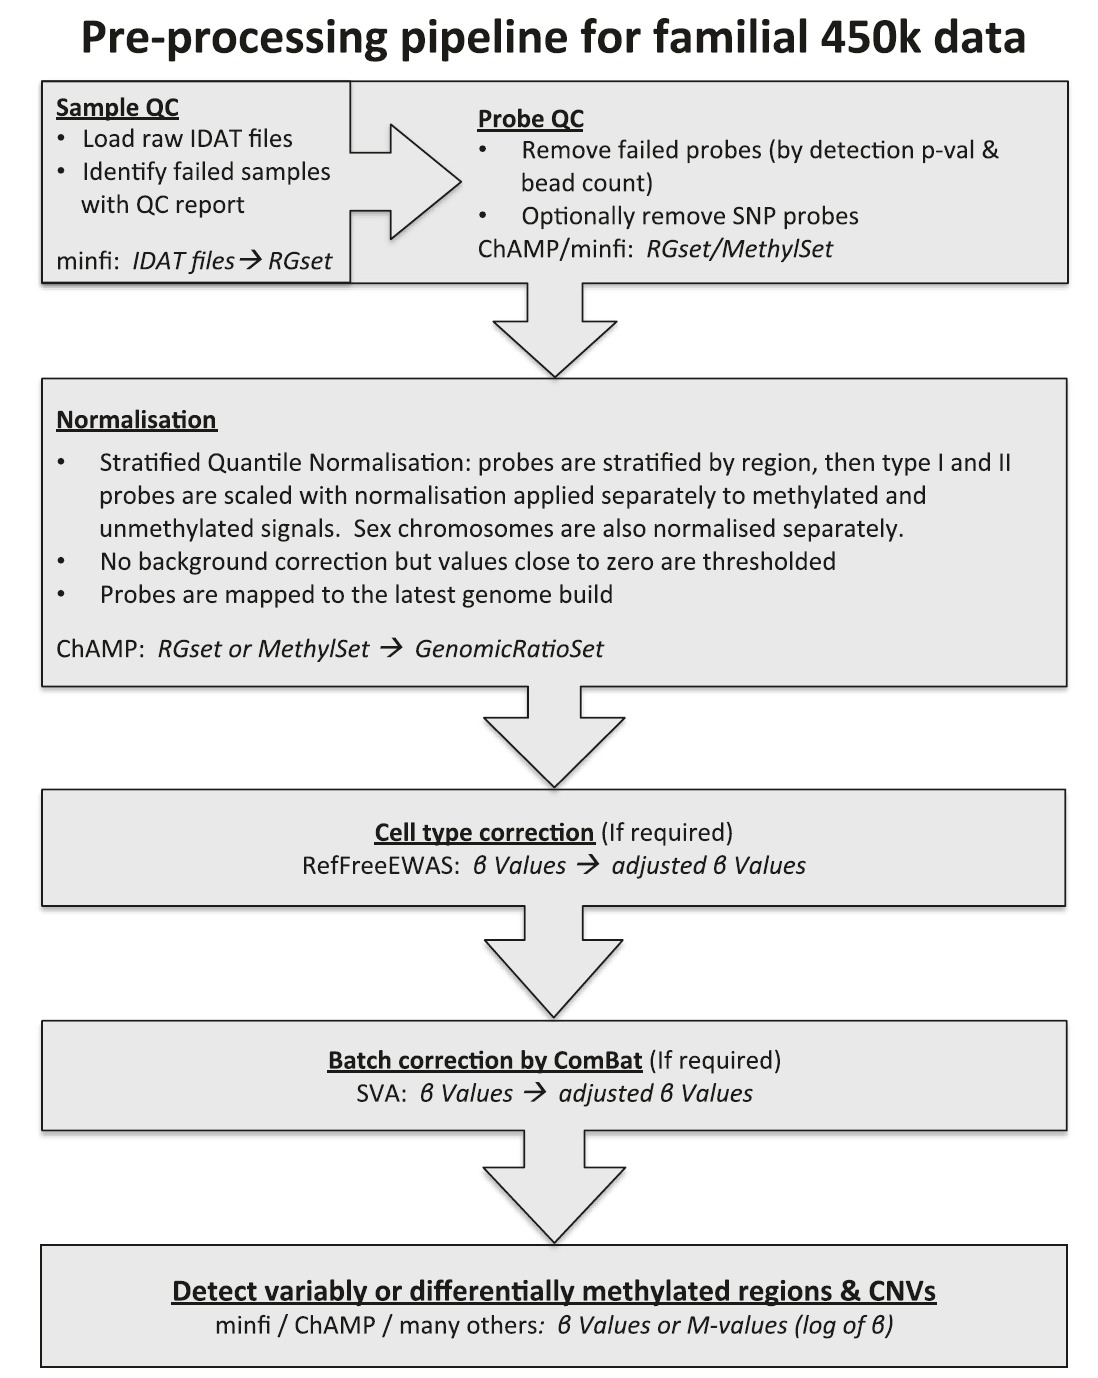
\includegraphics[width=0.5\linewidth]{Figures/Pipeline for familial data processed on the 450k array. Each box indicates a stage of the pipeline including the R package and the data.jpg}
  \caption{Pipeline for familial data processed on the 450k array. Each box indicates a stage of the pipeline including the R package and the data
format required/created in italics.}
  \label{fig:pipeline}
\end{figure}

\paragraph{Stratified Quantile Normalization Combined with ComBat}
Stratified Quantile Normalization (stratified QN) is an adaptation of the classical quantile normalization method designed to account for systematic technical variation in DNA methylation array data while preserving biologically meaningful differences across genomic contexts. In the standard quantile normalization, probe intensity distributions from all samples are forced to be identical, effectively removing unwanted variability but also potentially erasing real biological differences. Stratified QN mitigates this problem by performing normalization separately within predefined probe strata—typically defined by genomic features such as CpG islands, shores, shelves, and open sea regions. This stratification ensures that probes sharing similar biological and chemical properties are normalized together, thereby retaining context-specific methylation variability while minimizing within-array and between-array biases, particularly those arising from type I and type II probe design differences.

ComBat, on the other hand, is a batch correction algorithm based on an empirical Bayes framework that adjusts for systematic non-biological variation introduced by factors such as processing date, array batch, or laboratory conditions. ComBat models both location (mean) and scale (variance) batch effects and harmonizes data across batches while borrowing strength across all features to stabilize estimates, particularly in small sample sets. When applied after stratified QN, ComBat further eliminates residual inter-batch variability that persists even after normalization. The combined approach thus addresses two critical dimensions of technical bias: probe-specific intensity differences (handled by stratified QN) and batch-level heterogeneity (corrected by ComBat). This integration produces methylation datasets that are technically consistent yet biologically faithful, preserving inter-individual and familial epigenetic patterns essential for downstream analyses.


\paragraph{Results}
Among the tested methods, \textbf{stratified quantile normalization combined with ComBat} consistently outperformed others. Density plots revealed effective removal of within- and between-array bias, particularly the type I/II probe imbalance. MDS and clustering analyses confirmed that stratified QN + ComBat eliminated batch effects (p-value dropped from $<$0.01 to 0.97) while preserving familial clustering patterns. Quantitative metrics supported these findings: median absolute differences between replicates and DMRSE scores were lowest after applying this combined approach (DMRSE = 0.0012). Moreover, known biological associations—such as a methylation QTL at cg17749961—remained statistically significant (p = $1.05 \times 10^{-5}$) after normalization, indicating preservation of biological signal.

\paragraph{Discussion}
The paper emphasizes that normalization methods developed for case–control designs are unsuitable for familial data due to their reliance on dual-group assumptions. Stratified QN, based on genomic region stratification rather than inter-group contrasts, better retains subtle methylation variability within pedigrees. The addition of ComBat effectively mitigates batch-induced variance without distorting biological structure. The authors highlight the need for customized pipelines that integrate relationship-aware correction metrics to optimize methylation studies in complex familial or longitudinal datasets.

\paragraph{Conclusions}
A preprocessing workflow combining \textbf{stratified quantile normalization and ComBat batch correction} ensures high-quality, unbiased methylation profiles in the absence of control groups. This method balances technical correction with preservation of genuine biological differences, offering a reliable strategy for familial and multigenerational epigenetic analyses. The study establishes a reproducible framework for processing 450k array data where biological integrity and detection power must be maintained simultaneously.


\section{}

\section{}



\printbibliography

\end{document}
